\chapter{Simulation Frameworks}
\label{cha:frame}
Realistic simulations of IVC protocols are one of the main challenges in the VANET research domain. The ideal scenario is to perform an outdoor experiment, but setting up the vehicular network and running an outdoor experiment still has a high cost and potential safety issue. For example, in order to effectively evaluate the proposed system, we need many vehicles to communicate in a large road network, which may be costly and risky in real life.\\ In this field, network simulation environments, such as ns-3 and OMNeT++, are commonly used to model computer network configurations before they are deployed in the real world. Through simulation, the performance of different network setups can be compared, making it possible to recognize and resolve problems without conduct potentially expensive field tests.
As shown in \cite{mahajan2006urban} the quality of the results obtained by VANET simulations is heavily influenced by the quality of the mobility models.
\Cref{fig:mob} shown the evolution of mobility models \cite{sommer2008progressing}.
\begin{figure}[H]
    \centering
    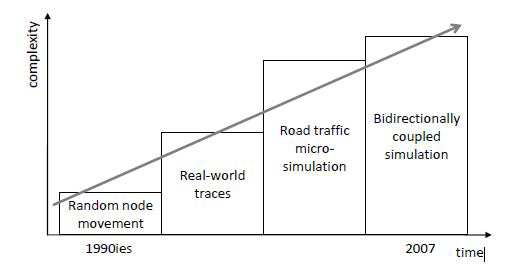
\includegraphics[width=0.7\textwidth]{fig/mobility.png}
    \caption{Evolution of mobility models}
    \label{fig:mob}
\end{figure}
Early approaches in mobility models relied on relatively simple models using random node movement \cite{johnson1996dynamic}.
Compared to the use of random mobility models, the modeling based on sets of pre-recorded real-world mobility trace was a crucial step towards realistic vehicle simulation. Such traces were obtained for example from the observation of city busses \cite{jetcheva2003design}. During network simulations, node mobility was controlled by synchronizing the position of the node in the simulation with the position of the vehicle stored in the trace file. \\
The difficulty on record trace data from real-world vehicle was overcame by generating movement traces artificially.
This way, artificial mobility models have the advantage of providing simulations with realistic mobility traces while at the same time allowing the freely adjustment of mobility parameters in order to understand their influence on simulations.\\
In case information about road congestion, accident, hazard warnings are transmitted over the network, a strictly interaction between the road traffic simulation and the network traffic is needed. \\
Bidirectionally coupled simulators like \cite{sommer2008need} provides not only more detailed insights into effects on network traffic, but at the same time have negligible impact on the run-time of simulations.
However, due to the on-the-fly node mobility computation,the results of the road traffic simulation cannot be re-used in form of trace files.
In bidirectional simulations, two inter-dependent processes are running concurrently, the network simulator and the road traffic simulator. The two processes share information like position and speed of the simulated nodes, while other data are local. The authors of \cite{sommer2008progressing} have analyzed the several mobility models and their impact.
In this thesis we decided to use Veins \cite{sommer2011bid} in combination with the network simulator OMNeT++ \cite{varga2001omnetpp} and the microscopic road traffic simulation package SUMO \cite{krajzewicz2002sumo}.
\section{Veins}
\label{sec:456}
Veins is an open source Inter-Vehicular Communication (IVC) simulation framework based on MiXiM \cite{kopke2008simulating} composed of an event-based network simulator and a road traffic micro simulation model. Both domains models are bi-directionally coupled and simulations are performed on-line. This way, not only the influence of road traffic on network traffic can be modelled, but also vice versa. In particular, the influences of IVC on road traffic can be modelled and complex interactions between both domains examined.\\
The framework is made up of two distinct simulators, OMNeT++ for network simulation and SUMO for road traffic simulation. \\
Veins includes a model of 802.11 that is tailored to use in vehicular networks, particularly IEEE 802.11p. This includes QoS channel access conforming to EDCA (that is, 4 queues with different access categories) and accurately captures frame timing, modulation and coding, and channel models.
Veins provides a comprehensive suite of IVC-specific models that can serve as a modular framework for simulating applications. Each model is contained in one or more of what OMNeT++ terms a \emph{module}, which can be instantiated in a running simulation to provide required functionality.
\section{Sumo}
\label{sec:Sumo}
Road traffic simulation models are classified into Macroscopic, Mesoscopic, and Microscopic models, according to the granularity with which traffic flows are examined. Macroscopic models model traffic at a large scale, while Mesoscopic model are concerned with the movement of whole platoons, using for example aggregated speed.density functions to model their behavior. However, simulations of VANETs scenarios are concerned with the accurate modelling of single radio transmission between a pair of nodes, so it require exact positions of simulated nodes. So, Mesoscopic and Macroscopic models cannot be used because they not offer this level of detail. \\
Traffic simulation in \emph{Veins} is performed by SUMO, which is a microscopic road traffic simulation package that uses the SK \cite{krauss1998microscopic} mobility model.
It can perform simulations both running with and without a GUI, and imports city maps from a variety of file formats.\\
SUMO allows high-performance simulations of huge networks with roads consisting of multiple lanes, as well as of intrajunction traffic on these roads, either using simple right-of-way rules or traffic lights. \\
Vehicle types are freely configurable with each vehicle following statically assigned routes, dynamically generated routes, or driving according to a configured timetable.
\section{OMNeT++}
OMNeT++ is a C++ based discrete event simulator for modeling communication networks, multiprocessors and other distributed or parallel systems. OMNeT++ is open-source, and it can be used either under the GNU General Public License or under its own license that also makes the software free for non-profit use.\\
Scenarios in OMNeT++ are represented by a hierarchy of reusable modules. Modules’ relationships and their communication links are stored as Network Description (NED) files and can be modeled graphically.\\ Typical ingredients of a NED description are simple module declarations, compound module definitions and network definitions. Simple module declarations describe the interface of the module: gates and parameters. Compound module definitions consist of the declaration of the module's external interface (gates and parameters), and the definition of sub-modules and their interconnection. A network definition basically defines a model as an instance of a module type. \\
Simulations are either run interactively, in a graphical environment, or are executed as command-line applications. The \emph{INET Framework} extension used in Veins, provides provides a set of OMNeT++ modules that represent various layers of the Internet protocol suite, e.g., the TCP, UDP, IPv4, and ARP protocols. It also provides modules that allow the modeling of spatial relations of mobile nodes and IEEE 802.11 transmissions between them.
\section{Connections}
\label{sec:Omnetpp}
\begin{figure}[H]
    \centering
    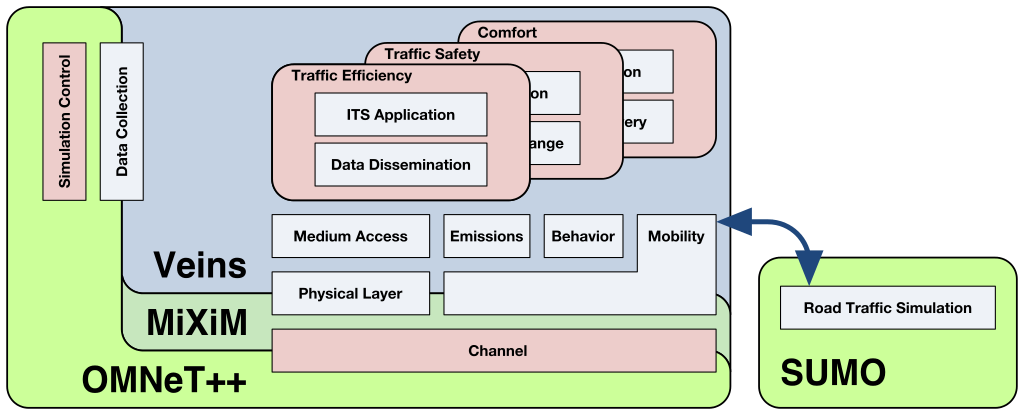
\includegraphics[width=0.7\textwidth]{fig/veins-arch.png}
    \caption{Structure of Veins}
\end{figure}
Each OMNeT++ node is associated with a network stack which includes an IEEE 802.11p wireless network interface provided by \emph{Veins}, plus a packet exchanging protocol and one or more applications.
To perform IVC evaluations, both simulators, OMNeT++ and SUMO, are running in parallel, connected via a TCP socket. \\The protocol for this communication has been standardized as the Traffic Control Interface (TraCI). This allows bi-directionally-coupled simulation of road traffic and network traffic. Movement of vehicles in the road traffic simulator SUMO is reflected in movement of nodes in an OMNeT++ simulation. Nodes can then interact with the running road traffic simulation, e.g. to simulate the influence of IVC on road traffic.\\
To do this, the control modules integrated with OMNeT++ and SUMO buffer any commands arriving within time steps in order to guarantee synchronous execution at each defined intervals. Every time step OMNeT++ then sends all commands to SUMO, at the end of the time step, SUMO would send a series of commands and the position of each vehicles to OMNeT++. Once it receive the commands it can reacts by introducing new nodes, by deleting the ones who had finished the simulation or by moving the nodes according to their road traffic simulation.\\
Using a simple request/response protocol, road traffic in SUMO can be influenced by OMNeT++ in different ways. Most importantly, time steps are generated to advance the simulation in SUMO. Furthermore, vehicles can be stopped to create artificial traffic jams, they can be resumed to
 resolve those jams, and each simulated vehicle can be individually rerouted around arbitrary road segments. This way, Veins accurately reflects how drivers that know about a traffic obstruction will try to avoid it. The sequence of messages exchanged between OMNeT++ and SUMO is shown in \Cref{fig:diagram}.
\begin{figure}[H]
    \centering
    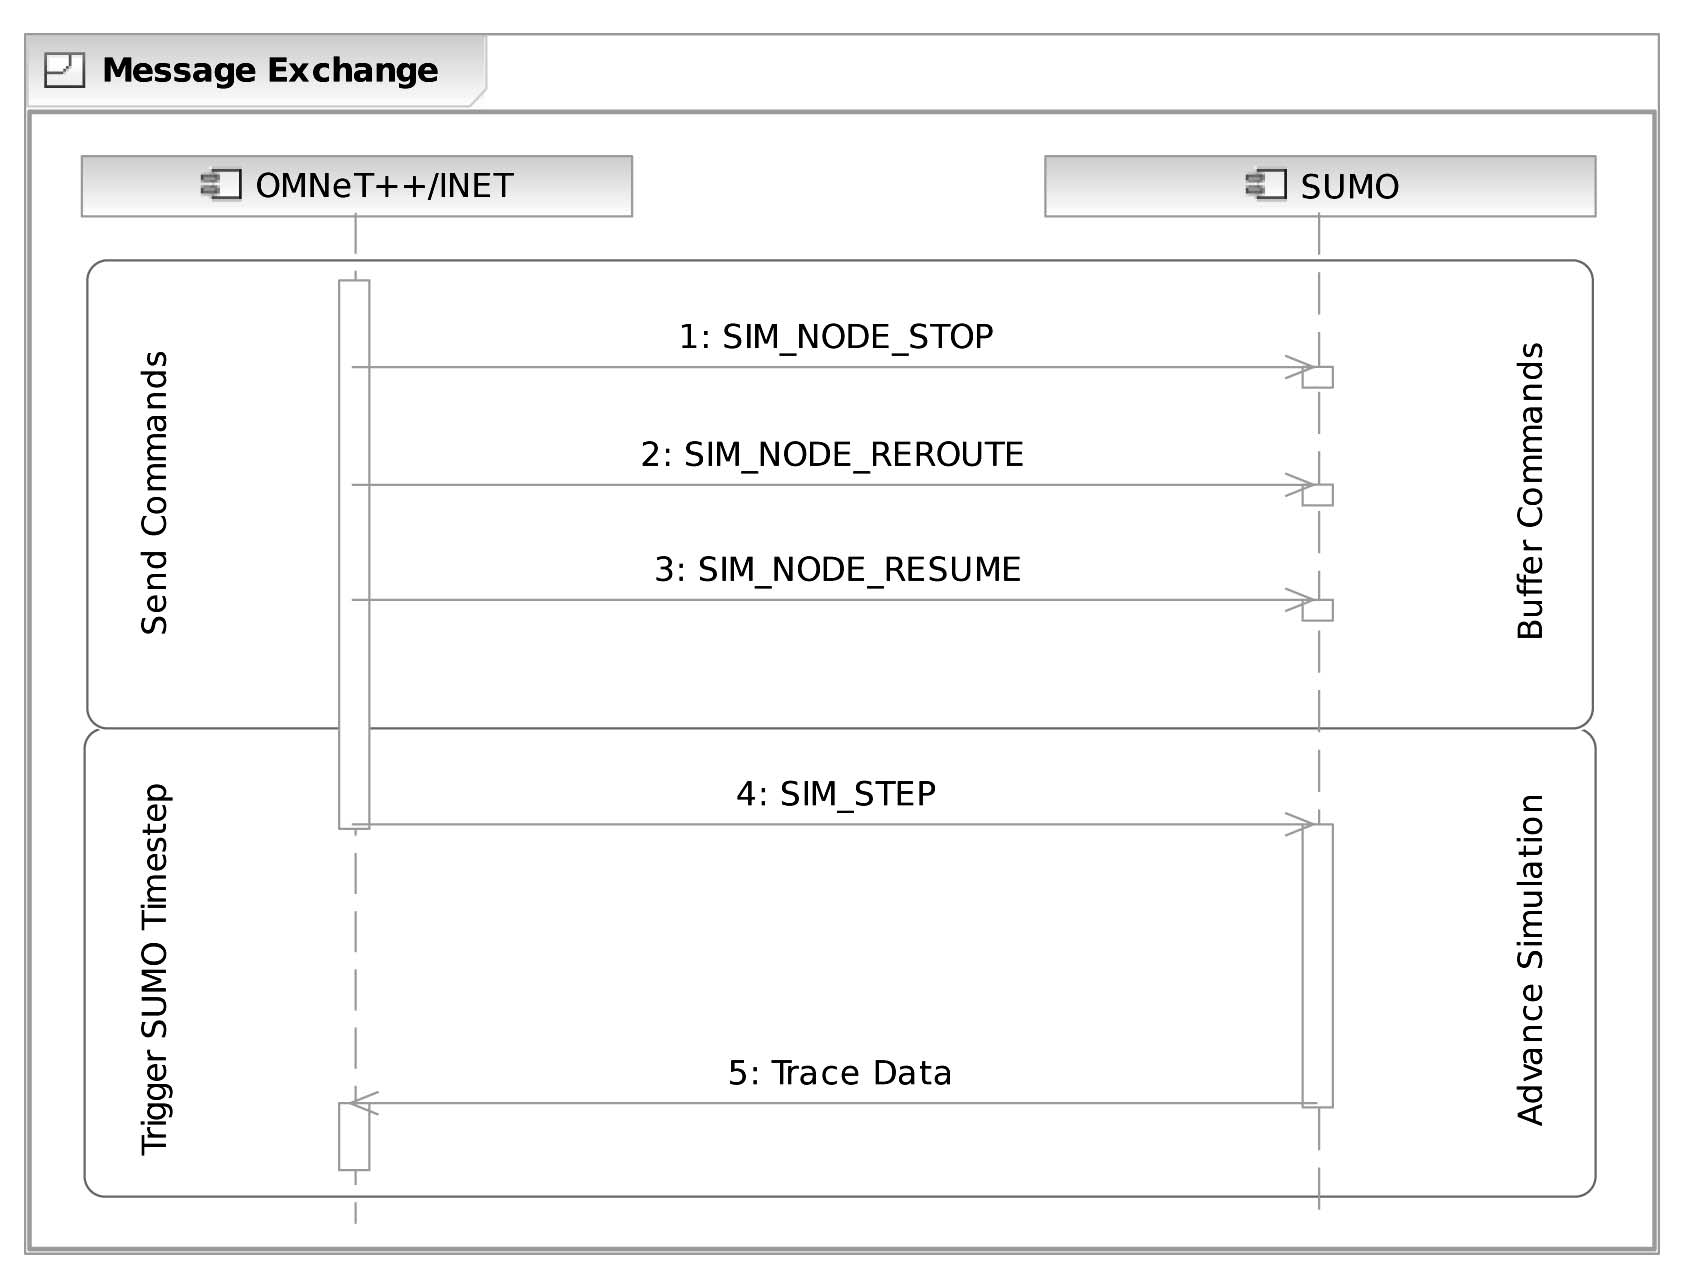
\includegraphics[width=0.7\textwidth]{fig/message-diagram.png}
    \caption{Sequence diagram of messages exchanged between network
    and road traffic simulator communication modules.}
    \label{fig:diagram}
\end{figure}
\newpage
